%%%%%%%%%%%%%%%%%%%%%%%%%%%%%%%%%%%%%%%%%
% University/School Laboratory Report
% LaTeX Template
% Version 2.0 (4/12/12)
%
% This template has been downloaded from:
% http://www.latextemplates.com
%
% License:
% CC BY-NC-SA 3.0 (http://creativecommons.org/licenses/by-nc-sa/3.0/)
%
% Original header:
%
% This is a LaTeX version of the sample laboratory report
% from Virginia Tech's copyrighted 08-09 CHEM 1045/1046 lab manual.
% Reproduction of this one appendix section for academic purposes
% should fall under fair use.
%
%%%%%%%%%%%%%%%%%%%%%%%%%%%%%%%%%%%%%%%%%

\documentclass{article}
\usepackage{graphicx}
\usepackage{float}
\usepackage{mathtools}

\title{ELEC 302-81\\ Lab 2\\ Transformer Fundamentals} % Title
% \author{John \textsc{Smith}} % Author name
\date{\today} % Specify a date for the report

\begin{document}

\maketitle

\begin{center}
  \begin{tabular}{lr}
    Date Performed: & January 28, 2013 \\
    Partners: & Rawley Dent \\
              & Charles Pittman \\
    Instructor: & Dr. Weatherford
  \end{tabular}
\end{center}

\pagebreak

%\setlength\parindent{0pt} % Removes all indentation from paragraphs

\section{Purpose of Experiment}
In this experiment, the basic characteristics of transformers were studied. Various transformer circuits 
with different unknown turns ratios were constructed in order to study the different voltage ratios at each particular 
turns ratio. Other transformer circuits were constructed to observe the similarity between the current ratio 
and turns ratio, and to observe the saturation curve of a magnetic circuit.

\section{Circuits Tested}
\subsection{Voltage Ratios}
\begin{figure}[H]
  \centering
  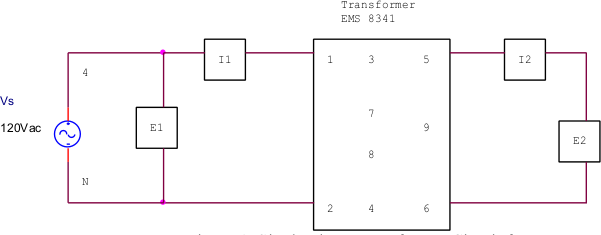
\includegraphics[width=.8\textwidth]{img/circuit_01}
  \caption{Single Phase Transformer Circuit}
  \label{fig:circuit_01}
\end{figure}

\subsection{Current Ratio}
\begin{figure}[H]
  \centering
  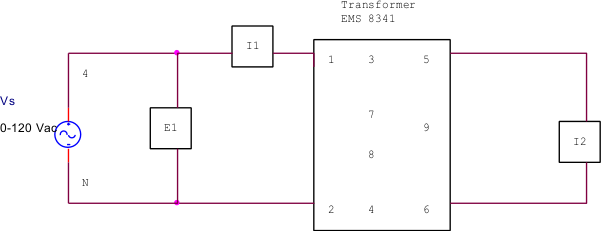
\includegraphics[width=.8\textwidth]{img/circuit_02}
  \caption{Single Phase Transformer Circuit}
  \label{fig:circuit_02}
\end{figure}

\subsection{Saturation}
\begin{figure}[H]
  \centering
  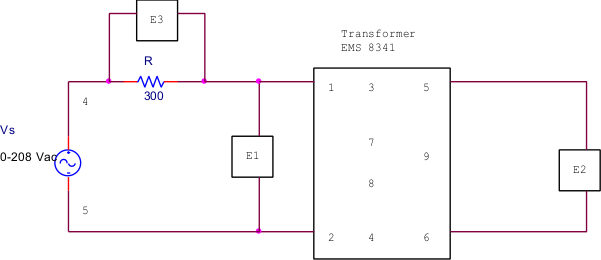
\includegraphics[width=.8\textwidth]{img/circuit_03}
  \caption{Single Phase Transformer Circuit}
  \label{fig:circuit_03}
\end{figure}

\section{Procedure}
\subsection{EMS Workstation Set-up}
At the Lab-Volt EMS workstation, a Fluke multi-meter was used to measure the DC resistance of each transformer
winding. These values are recorded in Table 1. The DAI 24-V supply was turned on, and the DAI USB connector was 
connected between the EMSworkstation and the PC. On the LVDAM EMS application software, the metering windows 
for E1, E2, E3, I1, and I2 were opened. The metering windows were set to continuous refresh. 

\subsection{Voltage Ratios}
\label{part1}
With the main power swtich to OFF and the voltage control knob fully counterclockwise (CCW), the voltmeter selector 
switch was set to postion 4-N. The circuit shown in Figure 1 was then constructed. The main power switch was
turned to ON and the voltage supply voltage was set to 120-V. The primary voltage was recorded from E1 and the 
secondary voltage was recorded from E2. The values for E1 and E2 were then measured and recorded for each winding
number listed in Table 2. The main power switch was set to OFF and the voltage control knob was set fully CCW
before rewiring the circuit for each winding number. The respective turns ratio for each set of winding 
number, primary, and secondary voltages was calculted and also listed in Table 2. After completing the requisite
measurements, the main power switch was set OFF and the voltage control to fully CCW.

\subsection{Current Ratio}
\label{part2}
The circuit shown in Figure 2 was then constructed. The main power switch was set ON and the voltage control knob
was slowly adjusted to read 0.4-A from I2. It was noted that the ammeter I2 shorted the windings 5-6. Hence,
extreme care was given to not exceed the secondary winding current rating of 0.5-A. The values for primary voltage
E1, primary current I1, and secondary current I2 were then measured and recorded, as shown in Table 3. The main 
power switch was set OFF and the voltage control knob fully CCW.

\subsection{Saturation}
\label{part3}
The circuit shown in Figure 3 was then constucted. The voltage supply connection was set from 4-N to 4-5. Since 
the exciting current was small the 300 ohm resistor was included and thus the voltage E3 across the resistor was 
used to show the current variation. On the PC, the Data Table application was opened and set to record settings 
from the Options tab. E1, E2, and E3 appeared as the columns in the data table. The main power switch was set ON 
and the supply voltage was then increased in 10-V increments from 0-180 volts. At each increment, the Record Data 
tab was clicked to instantly enter the voltage measurements in the data table. After reaching 180-V, the main power
switch was set to OFF and the voltage supply control knob was fully CCW. On the PC, the Graph application was opened. 
E3 (the excitiing current) was set as the x-axis, and E1 (the applied voltage) as the y-axis. The Line Graph tab was
clicked to display the saturation curve of the transformer core.

\section{Results}
\subsection{Voltage Ratios}
\begin{table}[H]
  \centering
  \begin{tabular}{cc}
    \hline
    Winding & Resistance \\
    \# & $\Omega$ \\
    \hline
    1--2 &  7.9 \\
    3--4 & 24.9 \\
    5--6 &  7.9 \\
    7--8 &  9.4 \\
    3--7 & 12. 1\\
    8--4 &  3.6 \\
    5--9 &  3.8 \\
    9--6 &  4.2 \\
  \end{tabular}
  \caption{Winding Resistances}
  \label{tab:wind_res}
\end{table}

\begin{table}[H]
  \centering
  \begin{tabular}{cccc}
    \hline
    Winding & Primary Voltage & Secondary Voltage & Turn Ratio \\
    \# & E$_1$ V (1--2) & E$_2$ V & N$_\text{P}$:N$_\text{S}$\\
    \hline
    3--4 & 120.3 & 207.2 & 0.58 \\
    5--6 & 120.2 & 119.2 & 1.01 \\
    7--8 & 120.2 &  75.8 & 1.59 \\
    3--7 & 120.3 & 103.6 & 1.16 \\
    8--4 & 120.3 &  27.8 & 4.33 \\
    5--9 & 120.2 &  59.8 & 2.01 \\
    9--6 & 120.1 &  59.7 & 2.01 \\
  \end{tabular}
  \caption{Primary and Secondary Voltages}
  \label{tab:volt_rat}
\end{table}

\subsection{Current Ratio}
\begin{table}[H]
  \centering
  \begin{tabular}{ccc}
    \hline
    E$_1$ & I$_1$ & I$_2$ \\
    V & A & A \\
    \hline
    11.75 & 0.403 & 0.399 \\
  \end{tabular}
  \caption{Winding Resistances}
  \label{tab:curr_rat}
\end{table}

\subsection{Saturation}
\begin{table}[H]
  \centering
  \begin{tabular}{ccc}
    \hline
    Primary Voltage & Secondary Voltage & Exciting Voltage\\
    E$_1$ V (1--2) & E$_2$ V & E$_2$ V\\
    \hline
    10.56 &  10.42 &  2.12 \\
    19.61 &  19.39 &  2.84 \\
    30.90 &  30.60 &  3.57 \\
    40.77 &  40.39 &  4.11 \\
    50.02 &  49.60 &  4.59 \\
    60.76 &  60.27 &  5.12 \\
    70.54 &  70.03 &  5.62 \\
    80.48 &  79.90 &  6.04 \\
    91.36 &  90.73 &  6.59 \\
    99.36 &  98.66 &  7.02 \\
    110.57 & 109.78 &  7.63 \\
    119.85 & 119.07 &  8.20 \\
    130.03 & 129.16 &  8.91 \\
    140.67 & 139.77 &  9.76 \\
    149.73 & 148.70 & 10.70 \\
    160.85 & 159.70 & 12.25 \\
    171.55 & 170.27 & 14.50 \\
    180.38 & 178.92 & 17.11 \\
  \end{tabular}
  \caption{Data for Fig~\ref{fig:circuit_03}}
  \label{tab:circuit_3}
\end{table}

\begin{figure}[H]
  \centering
  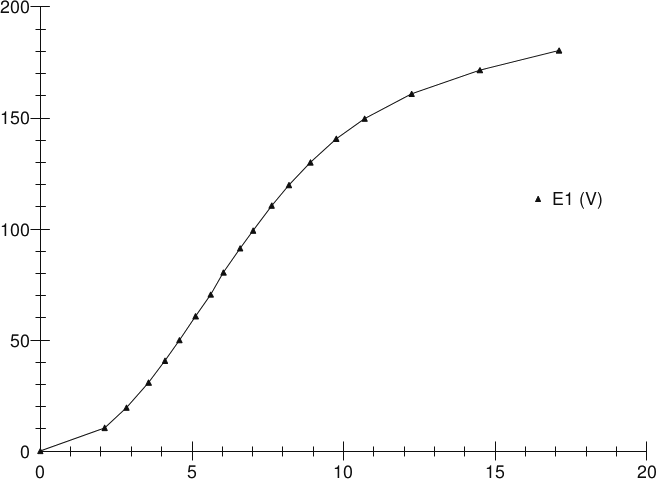
\includegraphics[width=.8\textwidth]{img/graph}
  \caption{Saturation Curve}
  \label{fig:graph}
\end{figure}

\section{Conclusions}
By measuring the resistance of each transformer winding and not getting any extremely high resistance 
readings similar to an open circuit, it was determined that the transformer windings had no faults and 
the integrity of the windings were intact.

By measuring the voltage ratios for each particular transformer winding, the turns ratio for that winding
was calculated by taking the primary voltage over the secondary voltage. This was one method to determine
the turns ratio of an unspecified transformer. 

By measuring the current ratio for one set of transformer windings, another method to determine the turns ratio
was implemented. By referring to the text \emph{Electric Machinery Fundamentals}, the current ratio of a 
transformer is inversely proportional to the turns ratio. The relationship states: \frac{Ip}{Is} = \frac{Ns}{Np}, 
where Ip is the primary current, Is the secondary current, Np the primary winding, and Ns the secondary winding. 
The ratio of secondary current I2 over primary current I1 was the same as the turns ratio calculated and recorded 
in row 2 of Table 2 pertaining to winding number 5-6. Therefore, the additional method of determing a transformer 
turns ratio was verified.

By analyzing the saturation curve, it was determined that the transformer core did indeed become saturated.
From an applied voltage of 10-V to approximately 110-V, the saturation curve was linear and the tranformer
core was unsaturated at this time. A small increase in the magnetomotive force (represented as E3) resulted in 
a very large increase in the flux produced (represented as E1). Then the saturation curve started to level off 
after an applied voltage of 110-V (termed the \emph{knee} of the curve), and therefore the core started to 
become saturated. In the saturated region, increases in magnetomotive force produce smaller and smaller increases 
in flux.

\end{document}
